\documentclass{article}
\usepackage{graphicx}
\usepackage[a4paper, total={6in, 8in}]{geometry}
\usepackage{amsmath}

\graphicspath{{./assets/}} % Specifies the directory where images are stored

\title{COMP579: Assignment 3}
\author{Jacqueline Wu, Sam Zhang}
\date{March 2024}

\begin{document}

\maketitle

\section{Value-based method with linear function approximation}
We implement Q-Learning and Expected SARSA and experiment them with in two environments from the Gymnasium, an open-source fork of the OpenAI Gym.\cite{gymnasium}
During the experiment, the environment's states are discretized through tile-coding into a binary vector, with a randomized offset for each tile.

\subsection{Methodologies}
We experiment with a fixed set of 3 different learning rates $\alpha \in \{ \frac{1}{4}, \frac{1}{8}, \frac{1}{16} \}$.
For each learning rate, we also experiment with 3 different $\epsilon$, where one 1 is an
exponentially decaying $\epsilon$ and the other 2 are fixed. We use decaying $\epsilon$ to
gauge the effect of encouraging exploration in the early stages of learning
and eliminating it in the later stages.

For each learning rate, we divide them by the number of tilings to avoid integer overflow during
the experiment.

\subsection{Results}

\begin{figure}[htbp]
    \centering
    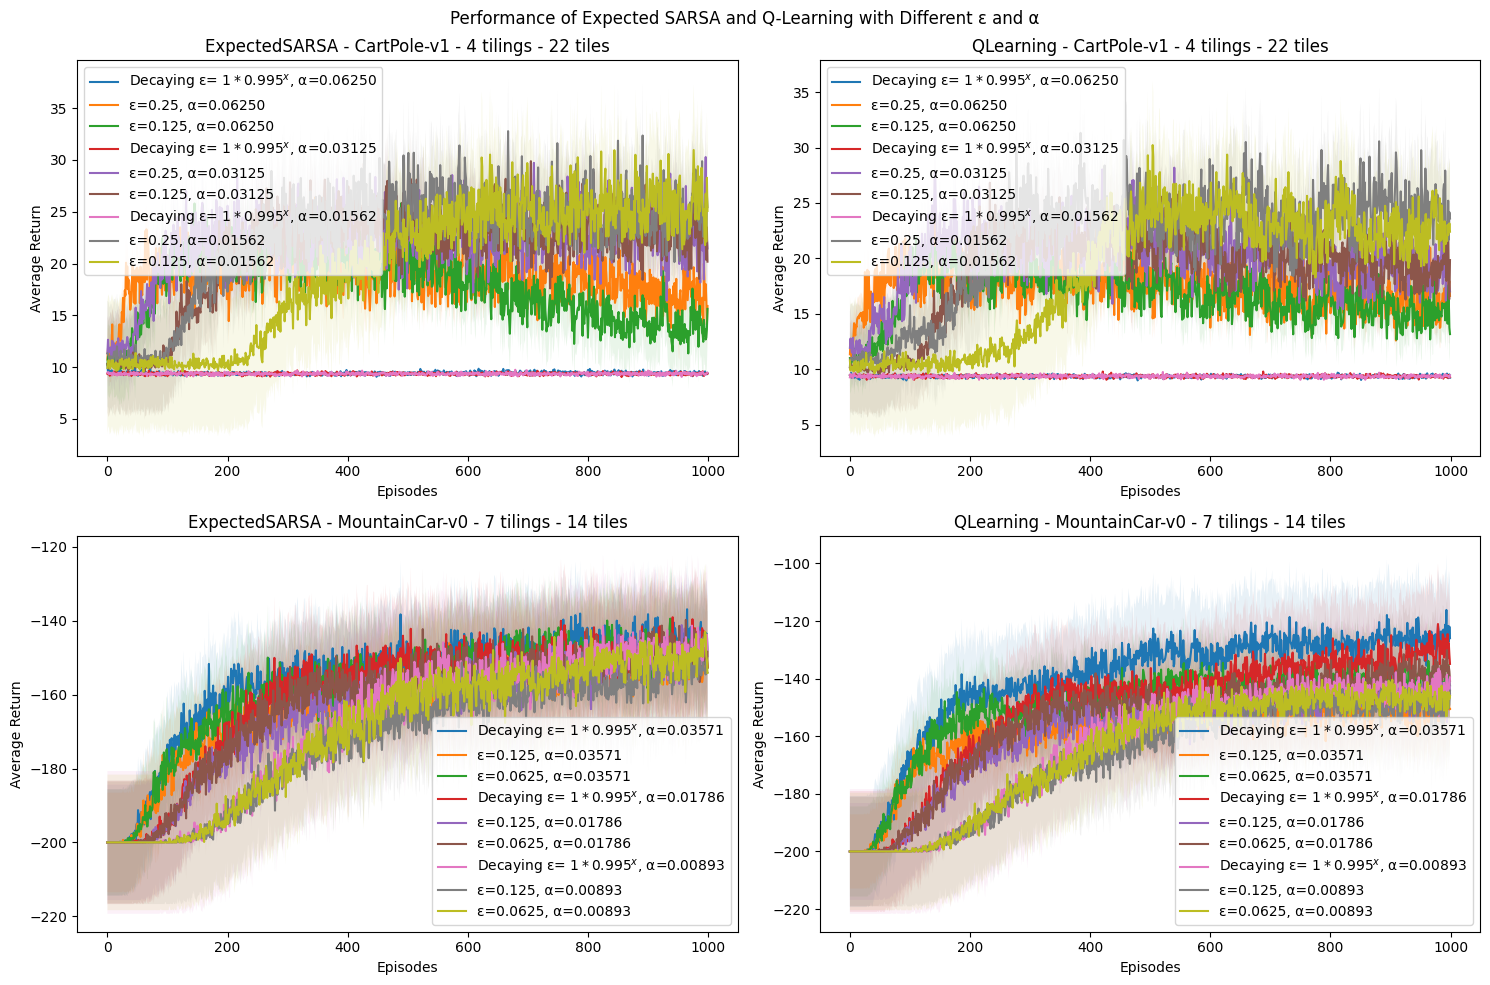
\includegraphics[scale=0.35]{q1.png}
    \caption{Mean reward per episode of ExpectedSARSA and Q-Learning on CartPole-v1 and MountainCar-v0}
    \label{fig:q1}
\end{figure}

The results of the experiments are shown in Figure \ref{fig:q1}, the values of $\alpha$ are
written post-division by the number of tilings.

we observe that both experiments learned CartPool-v1 poorly, and stops learning
early on, achieving rewards of sub-$30$. Out of all combinations, the best-performing combination for both
algorithms is $\alpha = \frac{1/16}{\text{number of tilings}}, \epsilon = 0.25$, where learning
happened the fastest and remained the most stable.

Both algorithms performed better on MountainCar-v0, with the best performing ExpectedSARSA achieving consistent rewards of
reward $\approx -150$, and Q-Learning achieving reward $\approx -130$. The best performing hyperparameters
combination for both algorithms is $\alpha = \frac{1/4}{\text{number of tilings}}, \epsilon = 1\times
0.995^{\text{episode}}$.

\subsection{Discussion}
We begin by highlighting the poor performance of value-based linear approximation on CartPole-v1. This is
the case for both algorithms and a wide range of hyperparameter combinations; no algorithm
stood out as being particularly better than the other, potentially due to the 4-dimensional state space being too complex for a linear approximation to capture.

The results do show a few characteristics with different hyperparameters, such as better stability with a
lower learning rate, and decaying $\epsilon$ preventing the model from learning at all, but
the takeaways are limited because this is not based on a great performance,
future experiments with more episodes, a different RL algorithm, or non-linear function approximation
may be suitable to attempt to achieve better results.

For MountainCar-v0, both algorithms performed better, with obvious patterns of learning and
stabilization, suggesting that linear function approximation is suitable.
Out of the two algorithms, the Q-Learning algorithm performed better than ExpectedSARSA in average reward.
This may imply that the environment is better suited for off-policy learning, potentially
because the risk of negative outcomes in the environment is not high.

It is also worth noting that a decaying $\epsilon$ performed noticeably better than fixed $\epsilon$
for the specific environment + Q-Learning combination, suggesting that encouraging exploration
in the early stages of learning may have led the model to establish a good understanding of the
optimal actions and their rewards, and then exploit this knowledge through learning towards that
optimal action via Q-Learning.

\subsubsection{Differences in Environments}
Apart from the algorithms and the hyperparameters, the two environments have shown some
contrasting differences as well. Decaying $\epsilon$ did not work at all for CartPole, whereas
it worked best in MountainCar. Cartpole performed best with a smaller learning rate, and
MountainCar performed best on its largest learning rate. These differences may stem from the
difference in complexity of the two environments; MountainCar is only a two-dimensional environment
that might see advantages in learning more abrubtly with large learning rates, Q-Learning, and large epsilons early, whereas CartPole is a four-dimensional environment
that may require more careful and refined learning that we were unable to achieve.

\section{Policy Gradient Theorem}

The gradient policy theorem states that
\[
\nabla_\theta J(\theta) = \mathbb{E}_{\pi} \left[ \nabla_{\theta} \log \pi_{\theta}(s, a) \cdot G_t \right]
\]









\section{Policy-based methods with linear function approximation}

\subsection{Methodologies}

Experimental methodologies were similar to Question 1, but we select a single learning rate per
algorithm and environment. For each algorithm (REINFORCE with baseline and ActorCritic) and environment, we experiment with a static temperature and a
exponentially decreasing temperature.

Learning rates for this question are not divided by the number of tilings, since we were not
required to use a set of fixed learning rates.

\subsection{Results}

\begin{figure}[htbp]
  \centering
  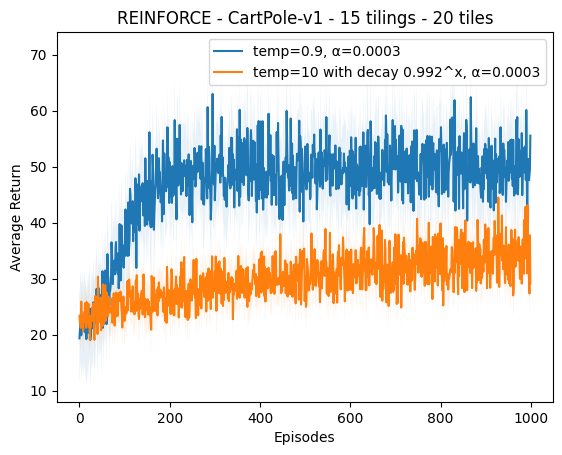
\includegraphics[width=0.41\textwidth]{q2_1.png}
  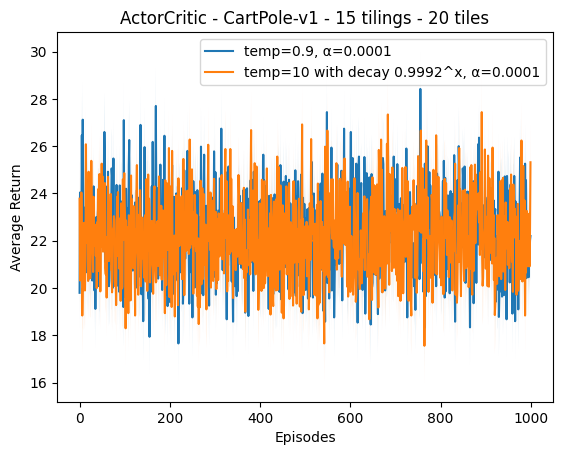
\includegraphics[width=0.41\textwidth]{q2_2.png}\\
  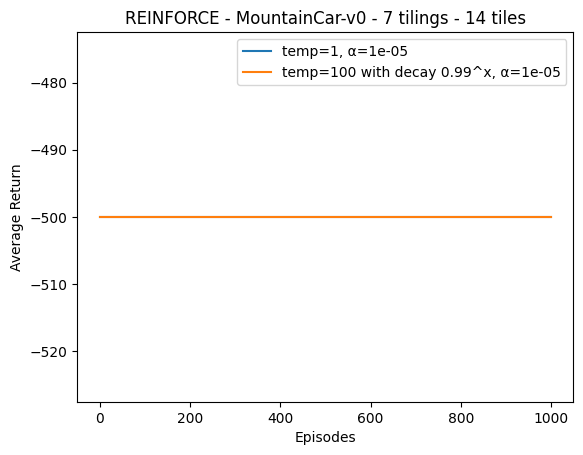
\includegraphics[width=0.41\textwidth]{q2_3.png}
  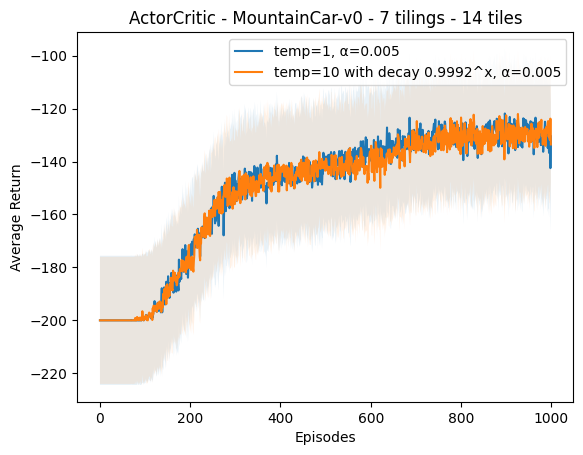
\includegraphics[width=0.41\textwidth]{q2_4.png}
  \caption{Mean reward per episode of REINFORCE and ActorCritic on CartPole-v1 and MountainCar-v0}\label{fig:q3}
\end{figure}

Figure \ref{fig:q3} showcases the results of the experiments with policy-based methods.

REINFORCE performed better than ActorCritic on CartPole-v1, achieving a mean reward of $\approx 50$, surpassing
value-based methods from Q1 as well. ActorCritic struggled to learn, achieving a mean reward of $\approx 25$,
similar to the value-based methods.

REINFORCE was entirely unable to learn MountainCar-v0, even with adjusted truncation step limit,
achieving a mean reward of $\approx -500$. ActorCritic performed better, achieving similar
results as the best performing value-based method, with a mean reward of $\approx -130$.

\subsection{Discussion}
Overall, policy-based methods did not performed significantly better than value-based methods,
with a minor exception on CartPole-v1 and REINFORCE showing a slight higher mean reward than
all other methods.

We highlight a few points of the environments observed in the results: notably, the non-linearity of
cartpole-v1 and the difficulty in learning the mountaincar-v0 environment with Monte-Carlo variants.
We observe that linear approximation

\subsubsection{Non-Linearity of CartPole-v1}

Through the results in this section and Question 1, we observe that linear approximation
for the CartPole-v1 environment has performed poorly all across the board, whether the algorithm
is value-based or policy-based. At best, we have been
able to achieve some learning in the early episodes using a few algorithms, but all algorithms
stabilized at sub-100 rewards, which is considered low given that the problem is considered solved at reward=190\cite{gym}.
This is a likely indication that the environment is too complex for a linear
approximation, particularly on states indicating a later part of the game.

One usefuly observation is that the REINFORCE algorithm, performed marginally better
than Actor-Critic, and methods from Q1 in the CartPole-v1 environment.
This performance edge could likely be attributed to REINFORCE's strategy of learning from complete trajectories,
allowing it to accumulate comprehensive experience from each episode.
This method of learning enables a more nuanced understanding of the cause-and-effect
relationship between actions and their long-term outcomes.

With these in mind, we conclude that linear approximation is sub-optimal
for the CartPole-v1 environment, but algorithms of Monte-Carlo variants may be useful for the general learning.
Future experiments should explore non-linear function approximation, perhaps with a focus on REINFORCE.


\subsubsection{Monte-Carlo Methods and MountainCar-v0}
We notice a severely poor performance of the Monte-Carlo method on MountainCar-v0,
despite achievements of decent rewards in the other methods of similar linear approximation. The method required
significantly more tuning and fine adjustments based on the nature of the environment,
such as a specific decreasing temperature algorithm.

This is unsurprising, notice that the environment's reward system state that
for each step that the car is not at the flag, the environment returns a reward of -1.
Given that Monte Carlo methods learned through an entire trajectory, a truncated
episode would result in a reward that provide little to no information about a good path to
reach the terminal state, as the algorithm learns from the \textbf{cumulative reward of completed episodes}.
Intuitively, a decreasing temperature would be helpful for the model to reach the terminal state, and then learn from early success runs.
But in practice, this has been extremely difficult to achieve, and the model has failed to learn
a policy to reach the terminal state.

Overall, with the positive results on other algorithms and the extra attention needed to tune the
REINFORCE algorithm, we conclude that Monte-Carlo variations are not desired for the MountainCar-v0 environment.
If we were to continue with the REINFORCE algorithm, experiments with larger
compute, notably with higher episodes and higher steps before truncation to successfully capture
a good amount of successful trajectories in the early stages would be helpful.

\newpage
\bibliography{ref}
\bibliographystyle{plain}
\end{document}
